\documentclass[10pt, a4paper]{article}
\usepackage[utf8]{inputenc}
\usepackage{amsmath}
\usepackage{amssymb}
\usepackage{amsthm}
\usepackage{parskip}
\usepackage{enumitem}
\usepackage{siunitx}
\usepackage{tikz}
\usepackage{pgfplots}
\usetikzlibrary{arrows.meta}
\usetikzlibrary{angles,quotes}
\pgfplotsset{compat = newest}

\title{Física Contemporánea\\Resolución de Tarea 1}
\author{Vite Riveros Carlos Emilio\\ Romero De La Rosa Gabriela Michelle\\ 
        Fisher Bautista Emir Julián\\ López Gallegos Fátima}
\date{23 septiembre del 2022}

\begin{document}
    \maketitle
    1. Problemas
    \begin{enumerate}
        \item El vector $\vec{a}$ tiene las componentes $(8, 14, 4)$ unidades respectivamente:
        
        \begin{center}
            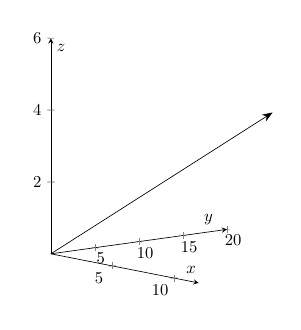
\begin{tikzpicture}[scale=.6]
                    \begin{axis}[
                        xlabel={$x$}, 
                        ylabel={$y$},
                        zlabel={$z$},
                        xmin=0, 
                        xmax=12, 
                        ymin=0, 
                        ymax=20, 
                        zmax=6,
                        zmin = 0, 
                        axis lines = middle,  
                        view = {50}{10}]
                        \addplot3[
                            -{Stealth[scale=1.3]}]table
                        {
                            x   y   z
                            0   0   0
                            8   14  4
                        };
                    \end{axis}
            \end{tikzpicture}
        \end{center}
        
       \begin{enumerate}
            \item Obtenga la expresión del vector $\vec{a}$ en términos de los vectores unitarios.
            \begin{center}
                $\vec{a_x}= \hat\imath(a_x)$\\
                $\vec{a_y}= \hat\jmath(a_y)$\\
                $\vec{a_z}= \hat{k}(a_z)$\\
                $\vec{a}= \vec{a_x}+\vec{a_y}+\vec{a_z}= \hat\imath(a_x)+\hat\jmath(a_y)+\hat{k}(a_z)$

                $\vec{a}= 8\hat\imath + 14\hat\jmath + 4\hat{k}$
            \end{center}

            \begin{center}
                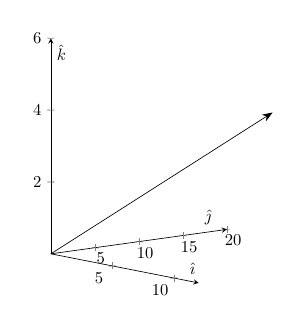
\begin{tikzpicture}[scale=.6]
                        \begin{axis}[
                            xlabel={$\hat\imath$}, 
                            ylabel={$\hat\jmath$},
                            zlabel={$\hat{k}$},
                            xmin=0, 
                            xmax=12, 
                            ymin=0, 
                            ymax=20, 
                            zmax=6,
                            zmin = 0, 
                            axis lines = middle,  
                            view = {50}{10}]
                            \addplot3[
                                -{Stealth[scale=1.3]}, black]table
                            {
                                x   y   z
                                0   0   0
                                8   14  4
                            };
                        \end{axis}
                \end{tikzpicture}
            \end{center}

            \item Determine una expresión para un vector $\vec{b}$ de $\frac{1}{4}$ de la longitud de $\vec{a}$ 
            apuntando en la misma dirección de $\vec{a}$.

            \begin{center}
                $\vec{b}= \frac{1}{4}(\vec{a})$\\
                $\vec{b}= \frac{1}{4}(\vec{a_x})+\frac{1}{4}(\vec{a_y})+\frac{1}{4}(\vec{a_z})$\\
                $\vec{b}= \frac{1}{4}(8)\hat\imath+\frac{1}{4}(14)\hat\jmath+\frac{1}{4}(4)\hat{k}$

                $\vec{b}= 2\hat\imath+3.5\hat\jmath+\hat{k}$
            \end{center}
            
            \begin{center}
                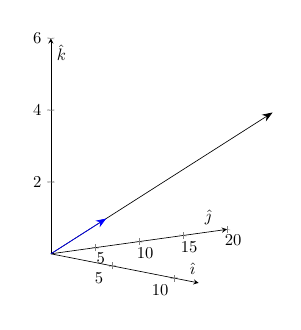
\begin{tikzpicture}[scale=.6]
                        \begin{axis}[
                            xlabel={$\hat\imath$}, 
                            ylabel={$\hat\jmath$},
                            zlabel={$\hat{k}$},
                            xmin=0, 
                            xmax=12, 
                            ymin=0, 
                            ymax=20, 
                            zmax=6,
                            zmin = 0, 
                            axis lines = middle,  
                            view = {50}{10}]
                            \addplot3[
                                -{Stealth[scale=1.3]}, black]table
                            {
                                x   y   z
                                0   0   0
                                8   14  4
                            };
                            \addplot3[
                                -{Stealth[scale=1.3]}, blue]table
                            {
                                x   y   z
                                0   0   0
                                2   3.5 1
                            };
                        \end{axis}
                \end{tikzpicture}
            \end{center}

            \item Calcule una expresión en términos de los vectores unitarios para un vector de
            tres veces la longitud de $\vec{a}$ apuntando en la dirección opuesta a la de él.

            \begin{center}
                $\vec{c}= -3(\vec{a})$\\
                $\vec{c}= (-3)\vec{a_x}+(-3)\vec{a_y}+(-3)\vec{a_z}$\\
                $\vec{c}= (-3)(8)\hat\imath + (-3)(14)\hat\jmath + (-3)(4)\hat{k}$

                $\vec{c}= -24\hat\imath + -42\hat\jmath + -12\hat{k}$
            \end{center}

            \begin{center}
                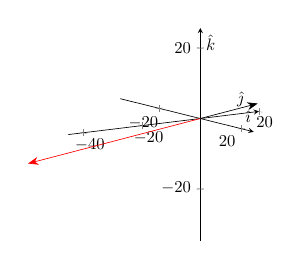
\begin{tikzpicture}[scale=.6]
                        \begin{axis}[
                            xlabel={$\hat\imath$}, 
                            ylabel={$\hat\jmath$},
                            zlabel={$\hat{k}$},
                            xmin=-25, 
                            xmax=12, 
                            ymin=-45, 
                            ymax=20, 
                            zmax=6,
                            zmin = -15, 
                            axis lines = center, 
                            axis equal, 
                            view = {55}{10}]
                            \addplot3[
                                -{Stealth[scale=1.3]}, black]table
                            {
                                x   y   z
                                0   0   0
                                8   14  4
                            };
                            \addplot3[
                                -{Stealth[scale=1.3]}, red]table
                            {
                                x   y   z
                                0   0   0
                                -24 -42 -12
                            };
                        \end{axis}
                \end{tikzpicture}
            \end{center}
       \end{enumerate}

       \item Un automóvil viaja hacia el Este con una rapidez de $50 \si{\frac{km}{h}}$. Está lloviendo
       verticalmente con respecto a la Tierra. Las marcas de la lluvia sobre las ventanas
       laterales del automóvil forman un ángulo de 60 grados con la vertical, calcule la
       velocidad de la lluvia con respecto a: (a) el automóvil y (b) la Tierra.

        \begin{center}
            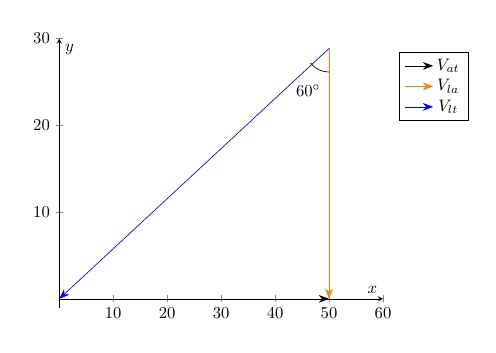
\begin{tikzpicture}[scale=.6]
                \pgfplotsset{every axis legend/.append style={ at={(1.05,0.95)}, anchor=north west,legend columns = 1}}
                \begin{axis}[
                    xlabel={$x$}, 
                    ylabel={$y$},
                    xmin=0, 
                    xmax=60, 
                    ymin=-1, 
                    ymax=30, 
                    axis lines = middle,  
                    view = {50}{10}]
                    \addplot[
                        -{Stealth[scale=1.3]}]table
                    {
                        x   y   
                        0   0
                        50  0
                    };
                    \addplot[
                        -{Stealth[scale=1.3]}, orange]table 
                    {
                        x   y
                        50  28.86
                        50  0
                    };
                    \addplot[
                        -{Stealth[scale=1.3]}, blue]table 
                    {
                        x   y
                        50  28.86
                        0  0
                    };
                    \coordinate (A) at (50, 27);
                    \coordinate (B) at (50, 28.86);
                    \coordinate (C) at (42, 25);
                    \pic [draw,-, black, angle eccentricity=2,"$\ang{60}$"] {angle = C--B--A};
                    \addlegendentry{$V_{at}$};
                    \addlegendentry{$V_{la}$};
                    \addlegendentry{$V_{lt}$};
                \end{axis}
            \end{tikzpicture}
        \end{center}

        \begin{center}
            Velocidad del automóvil: $V_{at}$\\
            Velocidad de la lluvia con respecto al automóvil: $V_{la}$\\
            Velocidad de la lluvia con respecto a la tierra: $V_{lt}$

            $V_{la}=\frac{V_{at}}{\sin{\ang{60}}}$\\
            $V_{la}=\frac{50\si{\frac{km}{h}}}{\sin{\ang{60}}}$

            $V_{la}= 57.73 \si{\frac{km}{h}}$

            $V_{lt}= \frac{V_{at}}{\tan{\ang{60}}}$\\
            $V_{lt}= \frac{50\si{\frac{km}{h}}}{\tan{\ang{60}}}$

            $V_{lt}= 28.86\si{\frac{km}{h}}$
        \end{center}

        \item Dos remeros en canoas idénticas ejercen el mismo esfuerzo remando en un río,
        uno corriente arriba (y se mueve corriente arriba), mientras que el otro rema
        directamente corriente abajo. Un observador en reposo sobre la orilla del río
        determina sus rapideces, $V_1$ y $V_2$ respectivamente. Determine, en términos de
        los datos conocidos, la rapidez del agua en el río.

        \begin{center}
            \begin{tikzpicture}[scale=.6]
                \pgfplotsset{every axis legend/.append style={ at={(1.05,0.95)}, anchor=north west,legend columns = 1}}
                \begin{axis}[
                    xlabel={$x$},
                    xmin=0, 
                    xmax=10, 
                    ymin=-1,
                    ytick={0},
                    xtick={0},
                    ymax=10, 
                    axis lines = middle,  
                    view = {50}{10}]
                    \addplot[
                        -{Stealth[scale=1.3]}]table
                    {
                        x   y   
                        10  2.5
                        5   2.5
                    };
                    \addplot[
                        -{Stealth[scale=1.3]}, red]table 
                    {
                        x   y
                        0   7.5
                        5   7.5
                    };
                    \addplot[
                        -{Stealth[scale=1.3]}, blue]table 
                    {
                        x   y
                        5   2.5
                        3  2.5
                    };
                    \addplot[
                        -{Stealth[scale=1.3]}, blue]table 
                    {
                        x   y
                        5   7.5
                        3   7.5
                    };
                    \addplot[
                        -{Stealth[scale=1.3]}, blue]table 
                    {
                        x   y
                        5   5
                        3   5
                    };                   
                    \addlegendentry{$\vec{p}$};
                    \addlegendentry{$\vec{q}$};
                    \addlegendentry{$\vec{r}$};
                \end{axis}
            \end{tikzpicture}
        \end{center}

        \begin{center}
            $V_1= \vec{q} -\vec{r}$\\
            $V_2= -(\vec{p} + \vec{r}$)\\
            $z = |\vec{q}| = |\vec{p}|$\\
            $V_1 = z - |\vec{r}|$\\
            $z = V_1 + |\vec{r}|$\\
            $V_2 = -(V_1 + |\vec{r}|) - |\vec{r}|$\\
            $V_2 = -V_1 - |\vec{r}| - |\vec{r}|$\\
            $V_2 = -V_1 - 2(|\vec{r}|)$\\
            $- 2(|\vec{r}|)= V_1 + V_2$

            $|\vec{r}|= -(\frac{V_1 + V_2}{2})$
        \end{center}
    \item Una persona se encuentra en la azotea de un edificio de $30 \si{m}$ de altura y lanza
    una piedra con una velocidad cuya magnitud es de $60 \si{\frac{m}{s}}$ con un ángulo de $\ang{33}$
    grados sobre la horizontal. Determine: (a) La altura máxima sobre la azotea
    alcanzada por la piedra, (b) La magnitud de la velocidad de la piedra justo antes
    de golpear el suelo, (c) La distancia horizontal de la base del edificio al punto
    donde la piedra golpea el suelo.

    \begin{enumerate}     
        \item    
        \begin{center}
            $\vec{V_0}= 60 \si{\frac{m}{s}}$, $\alpha = \ang{33}$\\
            $\vec{V_{0x}}= \vec{v_0} \cos{\alpha}= 60 \si{\frac{m}{s}} \cos{\ang{33}}$\\
            $\vec{v_{0x}}= 50.32 \si{\frac{m}{s}}$\\
            $\vec{v_{0y}}= \vec{v_0} \sin{\alpha} = 60 \si{\frac{m}{s}} \sin{\ang{33}}$\\
            $\vec{v_{0y}}= 32.67\si{\frac{m}{s}}$

            Supongamos $x_0=0$, $y_0=0$

            $y_{\text{max}}=\frac{|\vec{v_{0y}}|^2}{2g}=\frac{(32.67)^2}{2(9.81)}$

            $y_{\text{max}}=54.4 \si{m}$
        \end{center}
        \item 
        \begin{center}
            Cuando la piedra toca el suelo $y = -30$

            $y= y_0 + v_{0y}t-\frac{1}{2}(9.81)t^2$\\
            $-30= 0 + 32.67t-\frac{1}{2}(9.81)t^2$\\
            $0 = 30 + 32.67t-\frac{1}{2}(9.81)t^2$\\
            $t= \frac{-32.67 \pm \sqrt[]{32.67^2-4(30)(-\frac{1}{2}9.81)}}{2(-\frac{1}{2}9.81)}$\\
            $t=t_2=7.478 \si{s}$

            $v_y=v_{0y}-gt$\\
            $v_y=32.67-9.81(7.478)$\\
            $v_y=-40.689 \si{\frac{m}{s}}$\\
            $v_x=v_{0x}=50.32 \si{\frac{m}{s}}$\\
            $|v|=\sqrt[]{v_y^2+v_x^2}$\\
            $|v|=\sqrt[]{(-40.589)^2+(50.32\si{\frac{m}{s}})^2}$

            $|v|=64.713 \si{\frac{m}{s}}$
        \end{center}
        \item 
        \begin{center}
            $x=x_0+v_{0x}t$

            $x=0+50.32(7.478)$

            $x=376.29$
        \end{center}
    \end{enumerate}

    \item Se dispara un proyectil de modo que su alcance horizontal es igual al triple de
    la altura máxima. Encuentre el ángulo de lanzamiento.

    \begin{center}
        $y_{\text{max}}=\frac{|v_0|^2\sin^2{\alpha}}{2g}$\\
        $x_{\text{max}}=\frac{2|v_0|^2\cos^2{\alpha}}{g}$

        $\frac{3|v_0|^2\sin^2{\alpha}}{2g}=\frac{2|v_0|^2\sin\alpha\cos{\alpha}}{g}$\\
        $\frac{4}{3}=\frac{\sin\alpha}{\cos\alpha}$\\
        $\tan\alpha=\frac{4}{3}$\\
        $\tan^{-1}\frac{4}{3}=\alpha$

        $\alpha=\ang{53.13}$

        

    \end{center}

    \item Un lanza granadas tiene un alcance máximo de $300 \si{m}$. Para dar en un blanco
    que se encuentra a una distancia de $400 \si{m}$ del lanza granadas. Determine: (a) La
    rapidez de lanzamiento. (b) El ángulo de lanzamiento

        \begin{center}

            El alcance máximo se sabe que se da cuando $\theta = \ang{45}$, por ende:

            $\frac{|v_0|^2}{g}=300$, $\theta = \ang{45}$\\
            $|v_0|^2=(9.81)(300)$

            $|v_0|=54.249 \si{\frac{m}{s}}$

        \end{center}
    \end{enumerate}

    2. Preguntas

    \begin{enumerate}
        \item ¿Cuál sería la lectura en un velocímetro $3.5 \si{s}$ después de haberse dejado caer
        desde el reposo?

        \begin{center}
            $t= 3.5 \si{s}$\\
            $g= 9.8 \si{\frac{m}{s^2}}$\\
            $v= gt$\\
            $v= (9.8\si{\frac{m}{s^2}})(3.5\si{s})$

            $v= 34.335 \si{\frac{m}{s}}$
        \end{center}

        \item Si un automóvil se mueve con rapidez constante, ¿Se puede afirmar que también
        se mueve con velocidad constante? De un ejemplo apoyando su respuesta.

        No, un ejemplo sería un velocímetro de un automóvil que durante un intervalo de tiempo indique
        $60 \si{\frac{km}{h}}$ constantes, el velocímetro indica que la rápidez es constante, aunque la velocidad 
        no lo sea, ya que el automóvil podría no estarse moviendo en una trayectoria rectílinea, y podría 
        estar acelerando. :)

        \item ¿A que ángulo debería sujetarse una manguera de jardín para que la corriente
        de agua tenga un mayor alcance?

        \begin{center}
            A $\ang{45}$ debido que a $\ang{45}$ se tiene la distancia máxima.

            $x_m=\frac{|V_o|^2\sin{2x}}{g}$

            Si $x= \ang{45}$ entonces:

            $\sin{2x}=\sin{2(45)}=\sin{90}=1$
            
            Por lo tanto $\sin x = 1$ por esa razón el alcance máximo es cuando el ángulo es $\ang{45}$.
        \end{center}

        \item Escriba un ensayo acerca de la resistencia del aire de al menos una cuartilla.
        \begin{center}
            \textbf{La resistencia del aire}
        \end{center}
        Tendemos a dar por sentada la resistencia del aire (también conocida como "fricción").
        Suponemos que cuando lanzamos una pelota, un avión, una nave espacial o disparamos una
        bala, el viaje a través de la atmósfera es naturalmente más lento. Pero, ¿cuál es la razón detrás de
        esto? ¿Cómo puede el aire frenar un objeto, ya sea en caída libre o en vuelo?

        Por definición, tenemos que la resistencia del aire describe las fuerzas que se oponen al movimiento 
        relativo de un objeto cuando pasa por el aire. Estas fuerzas de resistencia actúan en sentido contrario 
        a la velocidad del flujo que se aproxima, frenando así el objeto. A diferencia de otras fuerzas de resistencia, 
        la resistencia aerodinámica depende directamente de la velocidad, ya que es el componente de la fuerza 
        aerodinámica neta que actúa en sentido contrario a la dirección del movimiento.

        Otra forma de decirlo sería decir que la resistencia del aire es el resultado de las colisiones de la 
        superficie principal del objeto con las moléculas de aire. Por lo tanto, se puede decir que los dos 
        factores más comunes que tienen un efecto directo sobre la cantidad de resistencia del aire son la 
        velocidad del objeto y el área de la sección transversal del objeto. Por lo tanto, tanto la velocidad como 
        el área de la sección transversal aumentan la resistencia del aire.

        Cuando un objeto cae, su velocidad inicial es cero. La caída libre puede ser un buen ejemplo. Cuando una 
        persona salta de un avión, no tiene movimiento horizontal, y su movimiento vertical se ve afectado por 
        la gravedad y el arrastre hacia arriba. Por lo tanto, la velocidad a la que la persona está cayendo es: la 
        velocidad es igual a negativo-g por tiempo. ¿Significa esto que la velocidad seguirá aumentando a medida que 
        el objeto siga cayendo hacia abajo?

        Después de algún tiempo, la fuerza de gravedad y la fuerza de arrastre hacia arriba ganan cantidades iguales. 
        Por tanto, la aceleración de la persona se detiene y la velocidad alcanza su máximo. La velocidad máxima de 
        caída se llama velocidad terminal.

        Siendo así que la velocidad terminal es el resultado de que la gravedad y el arrastre ascendente se equilibran 
        entre sí. Por ejemplo, un paracaidista en la posición habitual, es decir, con los brazos extendidos y mirando 
        al suelo, alcanza una velocidad terminal de unos 120 kilómetros por hora. Cuando se coloca un paracaídas abierto, 
        la velocidad terminal se reduce a 12 millas por hora, lo suficientemente lento como para aterrizar de pie y salir caminando.

        \item Considera una partícula que se mueve de manera análoga a una en tiro parabólico,
        pero con los efectos de rozamiento con el aire en ambas direcciones. Dibuje cualitativamente
        la trayectoria de la partícula si esta parte con una velocidad inicial horizontal $\vec{v_{x,0}}$. Explica 
        brevemente tu respuesta.

        \begin{center}
            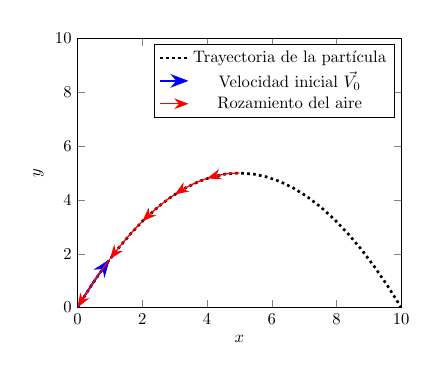
\begin{tikzpicture}[scale=.6]
                \begin{axis}[
                    xlabel={$x$},
                    ylabel={$y$},
                    xmin=0,
                    xmax=10,
                    ymin=0,
                    ymax=10
                ]
                    \addplot[dotted, ultra thick, domain=0:10] {-(.2*(x-5)^2-5)};
                    \addplot[-{Stealth[scale=1.3]}, samples = 10, domain=0:1, blue, very thick] {-(.2*(x-5)^2-5)};
                    \addplot[-{Stealth[scale=1.3]}, samples = 10, domain=1:0, red, thick] {-(.2*(x-5)^2-5)};
                    \addplot[-{Stealth[scale=1.3]}, samples = 10, domain=2:1, red, thick] {-(.2*(x-5)^2-5)};
                    \addplot[-{Stealth[scale=1.3]}, samples = 10, domain=3:2, red, thick] {-(.2*(x-5)^2-5)};
                    \addplot[-{Stealth[scale=1.3]}, samples = 10, domain=4:3, red, thick] {-(.2*(x-5)^2-5)};
                    \addplot[-{Stealth[scale=1.3]}, samples = 10, domain=5:4, red, thick] {-(.2*(x-5)^2-5)};
                    \addlegendentry{Trayectoria de la partícula}
                    \addlegendentry{Velocidad inicial $\vec{V_{0}}$}
                    \addlegendentry{Rozamiento del aire}

                \end{axis}
            \end{tikzpicture}
        \end{center}

        Tanto la velocidad como la resistencia del aire son proporcionales siendo así que mientras una sea más grande, la otra 
        también lo será.

        Como la resistencia del aire empuja al objeto hacia atrás, ya que es opuesta al movimiento, el vector resultante de sus 
        componentes es opuesto al vector de movimiento de la partícula.

    \end{enumerate}
\end{document}
